\section{Svetlo}

Viditeľné svetlo je forma energie pohybujúca sa v priestore, vzájomne pôsobiaca
s materiálmi, kde môže byť absorbovaná, lomená, odrazená alebo prenesená.

Ľudské oko dokáže zachytiť svetlo, ktorého výsledkom je stimulovanie oka k vytvoreniu
vizuálnych obrazov, závislých na vlnovej dĺžke. Vlnové dĺžky viditeľné ľudským okom
majú hodnoty od 380 do 780 nm. \cite{AHDR}

\subsection*{Rádiometria}

Veda zameraná na meranie svetla sa nazýva rádiometria. Pri meraní svetla nás zaujímajú
jeho vlastnosti šírenia priestorom, vzduchom, vodou a materiálmi. Energiu meriame v čase,
priestore alebo uhle.

\begin{description}
    % irradiance
    \item [Ožiarenie] je množstvo energie dopadajúce na jedno miesto z rôznych zdrojov a smerov.
    % radiance exitance
    \item [Žiarenie zdroja] je energia vyžarujúca z jedného bodu do všetkých prístupných smerov.
    % radiant intensity
    \item [Intenzita žiarenia] je energia vyžarovaná zo zdroja v jeden daný smer. Je meraná ako
    jednotka energie za jednotku času za jednotku uhlu smeru.
    % radiance
    \item [Žiarenie] je energia dopadajúca na jedno miesto z určitého smeru a v určitom uhle.
    Je to množstvo energie prenášané za jednotku času za jednotku plochy a za jednotku smeru.
\end{description}

\begin{figure}[h!]
    \centering
    \begin{subfigure}{0.2\textwidth}
        
\includegraphics[width=\textwidth]{figures/light/irradiance}
    \end{subfigure}
    ~
    \begin{subfigure}{0.2\textwidth}
        
\includegraphics[width=\textwidth]{figures/light/radiant_exitance}
    \end{subfigure}
    ~
    \begin{subfigure}{0.2\textwidth}
        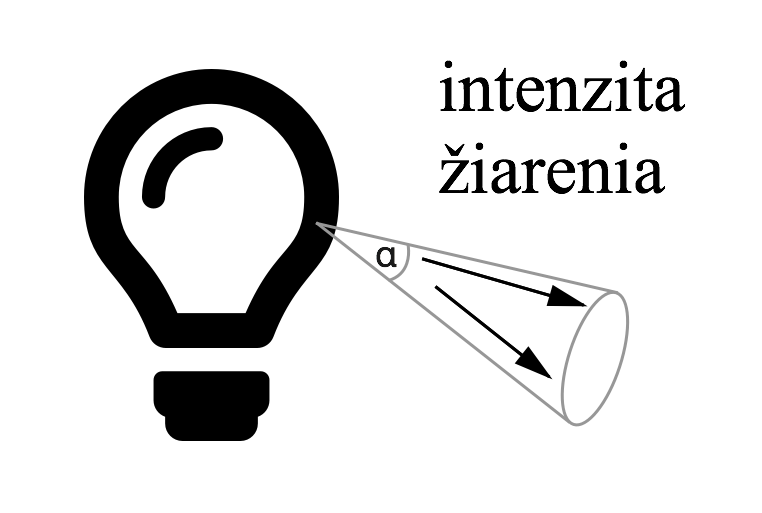
\includegraphics[width=\textwidth]{figures/light/radiant_intensity}
    \end{subfigure}
    ~
    \begin{subfigure}{0.2\textwidth}
        
\includegraphics[width=\textwidth]{figures/light/radiance}
    \end{subfigure}
    \caption{Rádiometrické veličiny}
    \label{fig:radiometry}
\end{figure}

Základým faktorom tvorby fotografie je svetlo dopadajúce na povrch z určitého smeru.
Pri vytváraní fotografie sa uzávierka fotoaparátu na malý čas otvorí a prepustí do vnútra 
fotoaparátu svetlo. Tomuto času hovoríme čas expozície. Dĺžka expozičného času určuje,
koľko svetla prenikne do tela fotoaparátu.
Šošovka fotoaparátu obmedzuje smer, z ktorého je svetlo prijímané.
Senzor je rozdelený na malé oblasti pixelov, kde každá oblasť zaznamená svetlo pre danú plochu.

\subsection*{Fotometria}

Fotometria je odbor optiky, ktorý skúma svetlo z pohľadu jeho pôsobenia na ľudské vnímanie.
Povrchy materiálov odrážajú svetlo a tým môžu pozmeniť jeho spektrálnu kompozíciu.
Následne odrazené svetlo nesie informáciu zároveň o zdroji svetla osvetľujúceho
povrch a~o~odrazivosti povrchu na danom mieste.

\begin{description}
    % luminosity
    \item [Svietivosť] je základnou fotometrickou veličinou. Svietivosť vyjadruje množstvo
    svetelného toku vyslaného zdrojom do priestorového uhla a je analogická intenzite žiarenia.
    % illuminance - osvetlenie
    \item [Osvetlenie] je definované ako svetelný tok dopadajúci na jednotku plochy a je analogické
    ožiareniu.
    % luminance
    \item [Jas] je fotometrická veličina vyjadrujúca intenzitu svietivosti pre jednotku plochy
    v určitom smere.
\end{description}

Jas kladie prirodzené hranice viditeľnosti vlnových dĺžok, čo je dôležité pre HDR.
Vlnové dĺžky nachádzajúce sa mimo rozsahu viditeľnosti nemusia byť zaznamenávané, ukladané a~ani
spracované. Základom väčšiny operátorov pre mapovanie tonality je počiatočné extrahovanie hodnôt
jasu každého pixelu podľa zložiek RGB pred zredukovaním dynamického rozsahu, pretože na vnímanie
majú väčší vplyv rozdiely v rozsahu jasu ako kontrast farieb.

\subsection*{Farebné priestory}

\begin{figure}[t]
    \centering
    \begin{subfigure}{0.54\textwidth}
        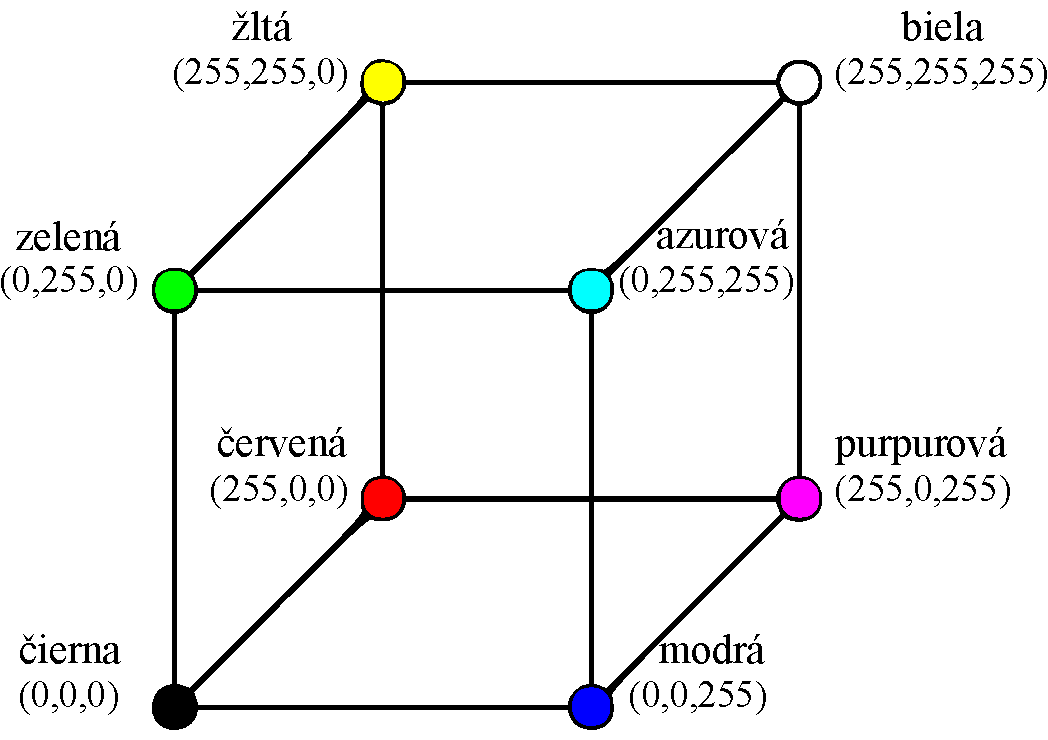
\includegraphics[width=\textwidth]{figures/light/rgb}
        \caption{RGB kocka}
        \label{fig:colorModels_rgb}
    \end{subfigure}
    ~
    \begin{subfigure}{0.35\textwidth}
        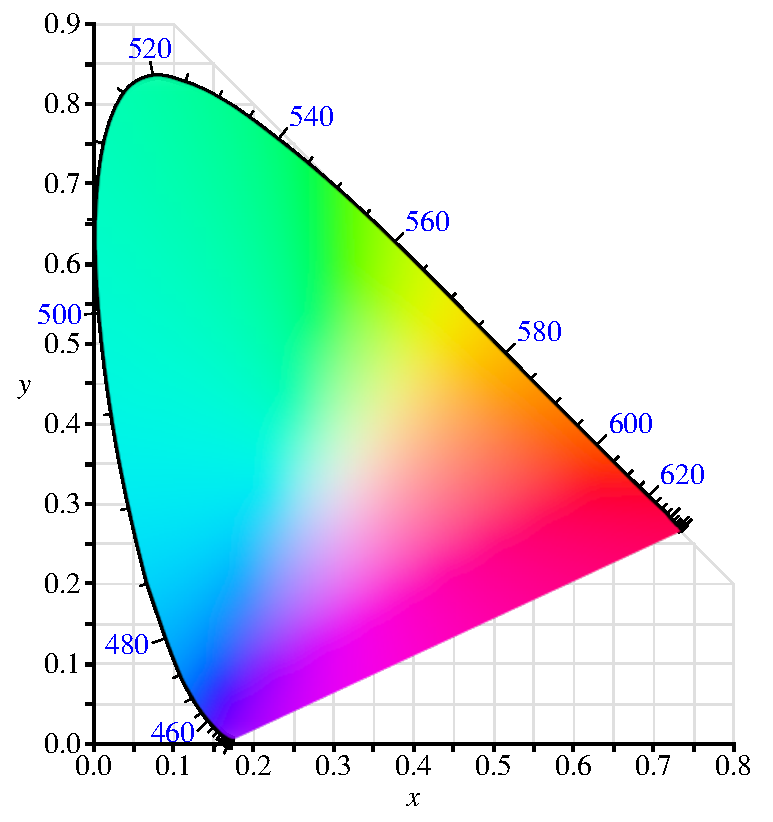
\includegraphics[width=\textwidth]{figures/light/cie}
        \caption{Chromatický diagram CIE}
        \label{fig:colorModels_cie}
    \end{subfigure}
    \caption{Grafická reprezentácia farebných priestorov \cite{AHDR}}
    \label{fig:colorModels}
\end{figure}

Farebný model popisuje reprezentáciu farieb ako $n$-ticu číselných hodnôt. Farba je väčšinou reprezentovaná troma alebo štyrmi farebnými
zložkami. Farebný priestor určuje rozsah farieb pre viditeľné spektrum.

\subsection*{sRGB}

Model RGB je založený na aditívnom miešaní primárnych farebných zložiek (červená, zelená a modrá), z ktorých každá stimuluje jeden z troch
farebných receptorov ľudského oka. Kombináciami týchto troch farebných zložiek obsiahneme značnú časť farebného priestoru, ktorý je človek
schopný vnímať. Žiaľ, neexistujú štandardy, ktoré by definovali aké hodnoty musia mať tieto základné farebné zložky, preto sa môžu rovnaké
hodnoty RGB na rozličných obrazovkách mierne líšiť. Farebný priestor tohoto modelu je možné reprezentovať v tzv. RGB kocke (obr.
\ref{fig:colorModels_rgb}). Akýkoľvek bod v kocke predstavuje farbu zloženú z farebných kanálov reprezentovaných 8 alebo 16-bitovou hodnotou.

\subsection*{CIE XYZ}

CIE XYZ je jedným z prvých matematicky definovaných farebných priestorov, ktorý je odvodený podľa vlastností ľudského oka. Každú farbu modelu
je možné presne matematicky popísať. Jedným spôsobom je popísať množstvo trichromatických zložiek, označovaných ako X, Y a Z. Výsledok dostaneme
integráciou spektrálneho farebného podnetu a trichromatických členov v celom rozsahu viditeľného spektra. Druhým spôsobom je vyjadriť 
tzv. trichromatické súradnice pomocou normových podielov.

V praxi sa využívajú na vyjadrenie chromatickosti farby iba zložky X a Y. V takom prípade je možné používať tzv. chromatický diagram (obr.
\ref{fig:colorModels_cie}).
